\documentclass[12pt,a4paper]{article}
\usepackage[utf8]{inputenc}
\usepackage[english,russian]{babel}
\usepackage{indentfirst}
\usepackage{misccorr}
\usepackage{graphicx}
\usepackage{amssymb}
\usepackage{amsmath}

\begin{document}

\begin{center}
    \large
    Работа 1.3.2
    
    Сибгатуллин Булат, Б01-007
    
    \vspace{0.5cm}
    \textbf{Определение модуля кручения}

\end{center}

\vspace{0.5cm}
\textbf{Цель работы:} измерение углов закручивания в зависимости от приложенного момента сил, расчет модулец кручения и сдвига при статистическом закручивании стержня, определение тех же модулей колебаний подвешенного на ней маятника (динамическим методом).

\vspace{0.5cm}
\textbf{В работе используются:} в первой части: исследуемый стержень, отсчетная трубка со шкалой, рулетка, микрометр, набор грузов; во второй части: проволока из исследуемого материала, грузы, секундомер, микрометр, рулетка, линейка.

\vspace{0.5cm}

При закручивании цилиндрических стержней круглого сечения распределение деформаций и напряжений одинаково только вдали от мест, где прикладываются закручивающие моменты. Для этих областей можно считать, что каждое поперечное сечение поворачивается как жесткое. Напряженнное состояние, которое при этом возникает, называется чистым кручением.

\begin{center}
    \large
    \textbf{I. Определение модуля кручения стержня статистическим}
\end{center}

\begin{figure}[h!]
\centering
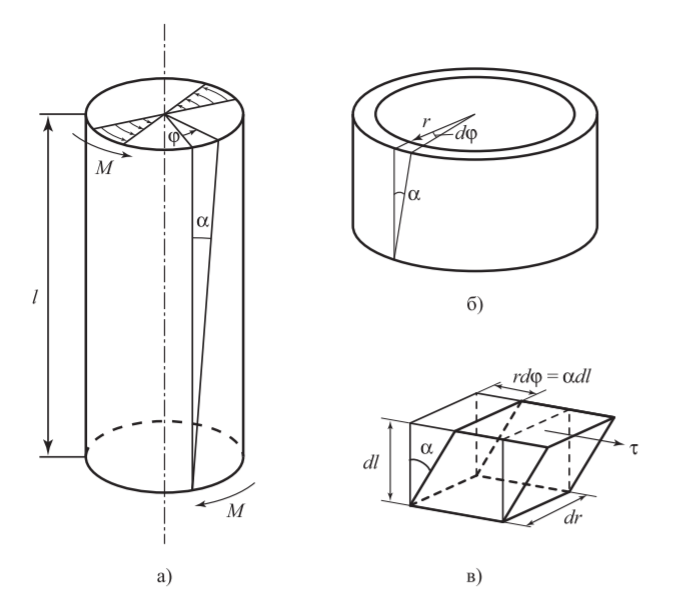
\includegraphics[scale=0.8]{Image1.png}
\caption{Закручивание цилиндра}
\label{fig:Image1}
\end{figure}

Рассмотрим часть закручиваемого круглого цилиндра, имеющую длину $l$, которая изображена на рис. 1а. Любая прямая линия, проведенная до закручивания цилиндра по частицам материала и параллельная оси симметрии, при закручивании превращается в спираль (винтовую линию). Сечения, находящиеся на расстоянии $l$, повернуты на угол $\varphi$.

Рассмотрим в цилиндре колечко произвольного радиуса $r$ с бесконечно малой высотой $dl$ и бесконечно малой толщиной $dr$ (рис. 1б). При закручивании верхнее сечение колечка поворачивается отночительно нижнего на угол $d\varphi$, а образующая цилиндрической поверхности колечка $dl$ наклоняется на угол $\alpha$, представляя элемент тех спиральных линий, о которых говорилось выше. При небольших углах $\alpha$ можно написать

\begin{equation}\label{1}
    \alpha dl = rd\varphi 
\end{equation}

Видно, что $\alpha$ возрастает с увеличением расстояния от оси цилиндра $r$. На рис. 1в показан элемент колечка, в котором происходит сдвиговая деформация. Касательное напряжение $\tau$ связано с углом сдвига $\alpha$ линейной зависимостью, в которую входит модель сдвига $G$:

\begin{equation}\label{2}
    \tau = G\alpha
\end{equation}

Касательное напряжение $\tau$ пропорционально $\alpha$ и, следовательно, тоже растет с увеличением расстояния от оси цилиндра, о чем уже говорилось выше. Используя (\ref{1}), получаем:
\begin{equation}\label{3}
    \tau = Gr\frac{d\varphi}{dl}
\end{equation}

Эти касательные напряжения создают момент сил относительно оси цилиндра:

\begin{equation}\label{4}
    dM = 2\pi rdr\cdot\tau\cdot r
\end{equation}

Суммарный момент сил, действующий на всем поперечном сечении цилиндра, находится интегрированием по колечкам от оси цилиндра до его радиуса $R$:

\begin{equation}\label{5}
    M = 2\pi G\frac{d\varphi}{dl}\int\limits_0^R r^3 dr = \pi G \frac{d\varphi}{dl}\frac{R^4}{2}
\end{equation}

Этот момент не меняется по длине цилиндра. Моменты на торцах любой выделенной части цилиндра уравновешивают друг друга (нет вращения цилиндра). При этом из (\ref{5}) следует линейная зависимость между относительным поворотом поперечных сечений цилиндра - углом $\varphi$ и расстоянием $l$, на котором они находятся. Таким образом, для связи приложенного момента сил $M$ и угла поворота $\varphi$ поперечных сечений цилиндра $\varphi$, находящихся на расстоянии $l$, получаем

\begin{equation}\label{6}
    M = \frac{\pi R^4 G}{2l}\varphi = f\varphi
\end{equation}

Здесь введен модульькручения $f$, связанный с модулем сдвига $G$:

\begin{equation}\label{7}
    f = \frac{\pi R^4 G}{2l}
\end{equation}

Необходимо подчеркнуть, что зависимость (\ref{6}) выполняется при напряжениях намного меньших модуля сдвига, то есть при малях углах $\alpha$.

\vspace{0,5cm}

\textbf{1.} Познакомимся с установкой, проверим, видно ли в зрительной трубе отражение шкалы в зеркальце. Измерим расстояние($l$) от зеркальца до шкалы, определим диаметр стержня($D$) и шкива($D_{\text{шк}}$).

\vspace{0,5cm}

\begin{tabular}{|c|c|c|c|c|c|c|c|c|c|c|}
\hline
$l$, см & 133,2 & 133,2 & 133,3 & 133,5 & 133,4 & 133,4 & 133,2 & 133,2 & 133,3 & 133,5 \\
\hline
$D$, мм & 5,95 & 5,93 & 5,95 & 5,95 & 5,94 & 5,95 & 5,94 & 5,95 & 5,95 & 5,94 \\
\hline
$R_{\text{шк}}$, см & 10,1 & 10,11 & 10,1 & 10,11 & 10,11 & 10,1 & 10,1 & 10,1 & 10,1 & 10,1 \\
\hline
\end{tabular}

\vspace{0,5cm}

Вычислим средние значения по формуле:

\begin{equation}\label{13}
l = \frac{1}{N} \sum\limits_{\textit{i} = 1}^N l_{\textit{i}}
\end{equation}

Здесь N - это количество измерений, тогда средние значения будут равны:

\[L = 133,32 \: \textit{см} \quad R = 2,973 \: \textit{мм} \quad R_{\text{шк}} = 10,103 \: \textit{см}\]

Систематические погрешности узнаем из характеристик приборо, а случайные вычислим по формуле:

\begin{equation}\label{14}
\sigma_l = \sqrt{\frac{1}{N} \sum\limits_{\textit{i} = 1}^N (l_{\textit{i}} - l)^2}
\end{equation}

\[\sigma_{l_{\text{сист}}} = 0,1 \: \textit{см} \quad \sigma_{l_{\text{сл}}} = 0,37\: \textit{см}\]

\[\sigma_{D_{\text{сист}}} = \sigma_{R_{\text{сист}}} =  0,01\: \textit{мм} \quad \sigma_{D_{\text{сл}}} = \sigma_{R_{\text{сл}}} = 0,002 \: \textit{мм} \]

\[\sigma_{R_{\text{шк сист}}} =  0,05\: \textit{мм} \quad \sigma_{R_{\text{шк сл}}} = 0,02 \: \textit{мм} \]

Зная случайные и систематические погрешности вычислим погрешности измерений по формуле:

\begin{equation}\label{15}
\sigma_l = \sqrt{\sigma{l_{\text{сист}}}^2 + \sigma_{l_{\text{сл}}}^2}
\end{equation}

\[\sigma_l = 0,38 \: \textit{см} \quad \sigma_{R_{\text{шк}}} = 0,054\:\textit{мм} \quad \sigma_R = 0,01 \: \textit{мм}\]

Увеличивая нагрузку на нитях снимем зависимость \textit{x} = \textit{x(m)}, где \textit{x}, смещение координат на шкале, отражающейся в зеркале, a \textit{m} масса груза, подвешенного на нити:

\vspace{0,5cm}

\begin{tabular}{|c|c|c|c|c|c|c|c|}
\hline
$m$, г & 198 & 396 & 594 & 792 & 594 & 396 & 198 \\
\hline
$x$, см & 9,4 & 17,8 & 26,5 & 34,8 & 27,9 & 17,8 & 9,1 \\
\hline
$x$, см & 9,1 & 17,8 & 26 & 36 & 28 & 17,7 & 9,4 \\
\hline
$x$, см & 9,1 & 17 & 26 & 35 & 27,2 & 17,2 & 9,2 \\
\hline
$x$, см & 9,2 & 17,6 & 25,7 & 34,9 & 28,3 & 17,9 & 9 \\
\hline
\end{tabular}  

\vspace{0,5cm}

Зная \textit{x} и \textit{l} можем посчитать угол $\varphi$ по формуле:

\[ \tan \varphi = \frac{x}{l}\]

По полученным данным построим зависимоть $\varphi = \varphi(\textit{M})$, где $ \textit{M} = \textit{mg}\textit{R}_{\text{шк}}$:

\vspace{0,5cm}

\begin{tabular}{|c|c|c|c|c|c|c|c|}
\hline
$M$, $\text{Н} \cdot \text{м}$ & 0,1962 & 0,3925 & 0,5887 & 0,7850 & 0,5887 & 0,3925 & 0,1962 \\
\hline
$\varphi_1$, рад& 0,0704 & 0,1327 & 0,1962 & 0,2553 & 0,2062 & 0,1327 & 0,0681 \\
\hline
$\varphi_1$, рад& 0,0681 & 0,1327 & 0,1926 & 0,2637 & 0,2070 & 0,1320 & 0,0704 \\
\hline
$\varphi_1$, рад& 0,0681 & 0,1268 & 0,1926 & 0,2567 & 0,2013 & 0,1283 & 0,0689 \\
\hline
$\varphi_1$, рад& 0,0689 & 0,1312 & 0,1904 & 0,2560 & 0,2092 & 0,1335 & 0,0674 \\
\hline
\end{tabular}

\vspace{0,5cm}

Вычислим средние значения $\varphi_1$ по формуле (\ref{13}), для каждого момента сил, и построим таблицу:

\vspace{0,5cm}

\begin{tabular}{|c|c|c|c|c|c|c|c|}
\hline
$M$, $\text{Н} \cdot \text{м}$ & 0,1962 & 0,3925 & 0,5887 & 0,7850 & 0,5887 & 0,3925 & 0,1962 \\
\hline
$\varphi_1$, рад& 0,0688 & 0,1309 & 0,1930 & 0,2579 & 0,2059 & 0,1316 & 0,0687 \\
\hline
\end{tabular}

\vspace{0,5cm}

Угол $\varphi$ используемый в формуле (\ref{6}) равен:

\[\varphi = \frac{\varphi_1}{2}\]

Тогда построим аналогичную таблицу для угла $\varphi$:

\vspace{0,5cm}

\begin{tabular}{|c|c|c|c|c|c|c|c|}
\hline
$M$, $\text{Н} \cdot \text{м}$ & 0,1962 & 0,3925 & 0,5887 & 0,7850 & 0,5887 & 0,3925 & 0,1962 \\
\hline
$\varphi$, рад& 0,0344 & 0,0655 & 0,0965 & 0,1290 & 0,1030 & 0,659 & 0,0344 \\
\hline
\end{tabular}

\vspace{0,5cm}

Погрешность момента сил определяется только погрешностью измерения $R_{\text{шк}}$ и равна:

\[\sigma_M = M_\text{ср}\cdot \frac{\sigma_{R_{\text{шк}}}}{R_{\text{шк}}} = 0,0017 \:\text{Н} \cdot \text{м}\]

Погрешность измерения $\varphi$ будет складываться из случаной и систематической погрешности. Случайную погрешность можем определить по формуле (\ref{14}), а систематическую погрешность по формуле:

\[\frac{\sigma_{\varphi_{\textit{сист}}}}{\varphi} = \sqrt{\Big( \frac{\sigma_x}{x}
\Big) ^2 + \Big( \frac{\sigma_l}{l} \Big) ^2}\]

\vspace{0,5cm}

\begin{tabular}{|c|c|c|c|c|c|c|c|}
\hline
$M$, $\text{Н} \cdot \text{м}$ & 0,1962 & 0,3925 & 0,5887 & 0,7850 & 0,5887 & 0,3925 & 0,1962 \\
\hline
$\sigma_{\varphi_{\textit{сист}}} $, рад& 4,2$\cdot 10^{-4}$ & 5,3$\cdot 10^{-4}$ & 6,6$\cdot 10^{-4}$ & 8,2$\cdot 10^{-4}$ & 6,9$\cdot 10^{-4}$ & 5,3$\cdot 10^{-4}$ & 4,2$\cdot 10^{-4}$ \\
\hline
$\sigma_{\varphi_{\textit{сл}}} $, рад& 9,4$\cdot 10^{-4}$ & 24,2$\cdot 10^{-4}$ & 20,8$\cdot 10^{-4}$ & 33,7$\cdot 10^{-4}$ & 28,9$\cdot 10^{-4}$ & 19,9$\cdot 10^{-4}$ & 11,2$\cdot 10^{-4}$ \\
\hline
\end{tabular}

\vspace{0,5cm}

Погрешность $\sigma_{\varphi}$ найдем по формуле:

\[\sigma_{\varphi} = \sqrt{\sigma_{\varphi_{\text{сл наиб}}} + \sigma_{\varphi_{\text{сист наиб}}}} = 0,0035 \:\text{рад}\]

При помощи метода наименьших квадратов построим график зависимости $\varphi = \varphi(\textit{M})$:

\[\varphi = k\textit{M}\],

Где $k$ найдем по формуле:

\[k = \frac{\langle M \varphi \rangle}{\langle M^2 \rangle} = \frac{0,081}{0,242} = 0,161 \]

По формуле (\ref{6}) определим значение $\textit{f}$:

\[\textit{f} = \frac{1}{k} = 6,253 \: \text{Н} \cdot \text{м}\]

Погрешность $\textit{f}$ будет находиться по формуле:

\[\sigma_{\textit{f}} = \textit{f}\sqrt{\Big(\frac{\sigma_{\varphi}}{\varphi_{\text{ср}}}\Big)^2 + \Big(\frac{\sigma_{M}}{M}\Big)^2} = 0,015 \: \text{Н} \cdot \text{м}\]

Используя формулу (\ref{7}) вычислим значение модуля сдвига \textit{G}:

\[\textit{G} = \frac{6,253 \cdot 2 \cdot 1,3332}{(2,973 \cdot 10^{-3})^4 \cdot 1,1415} = 6,791 \cdot 10^{10} \: \text{Н}/\text{м}^2\]

И погрешность модуля сдвига рассчитаем по формуле:

\[\sigma_{\textit{G}} = \textit{G}\sqrt{\Big(\frac{\sigma_{\textit{f}}}{\textit{f}}\Big)^2 + \Big(\frac{\sigma_{\textit{l}}}{\textit{l}}\Big)^2 + 4\Big(\frac{\sigma_{\textit{R}}}{\textit{R}}\Big)^2} = 2,87 \cdot 10^8 \: \text{Н}/\text{м}^2\]

\begin{figure}[h!]
\centering
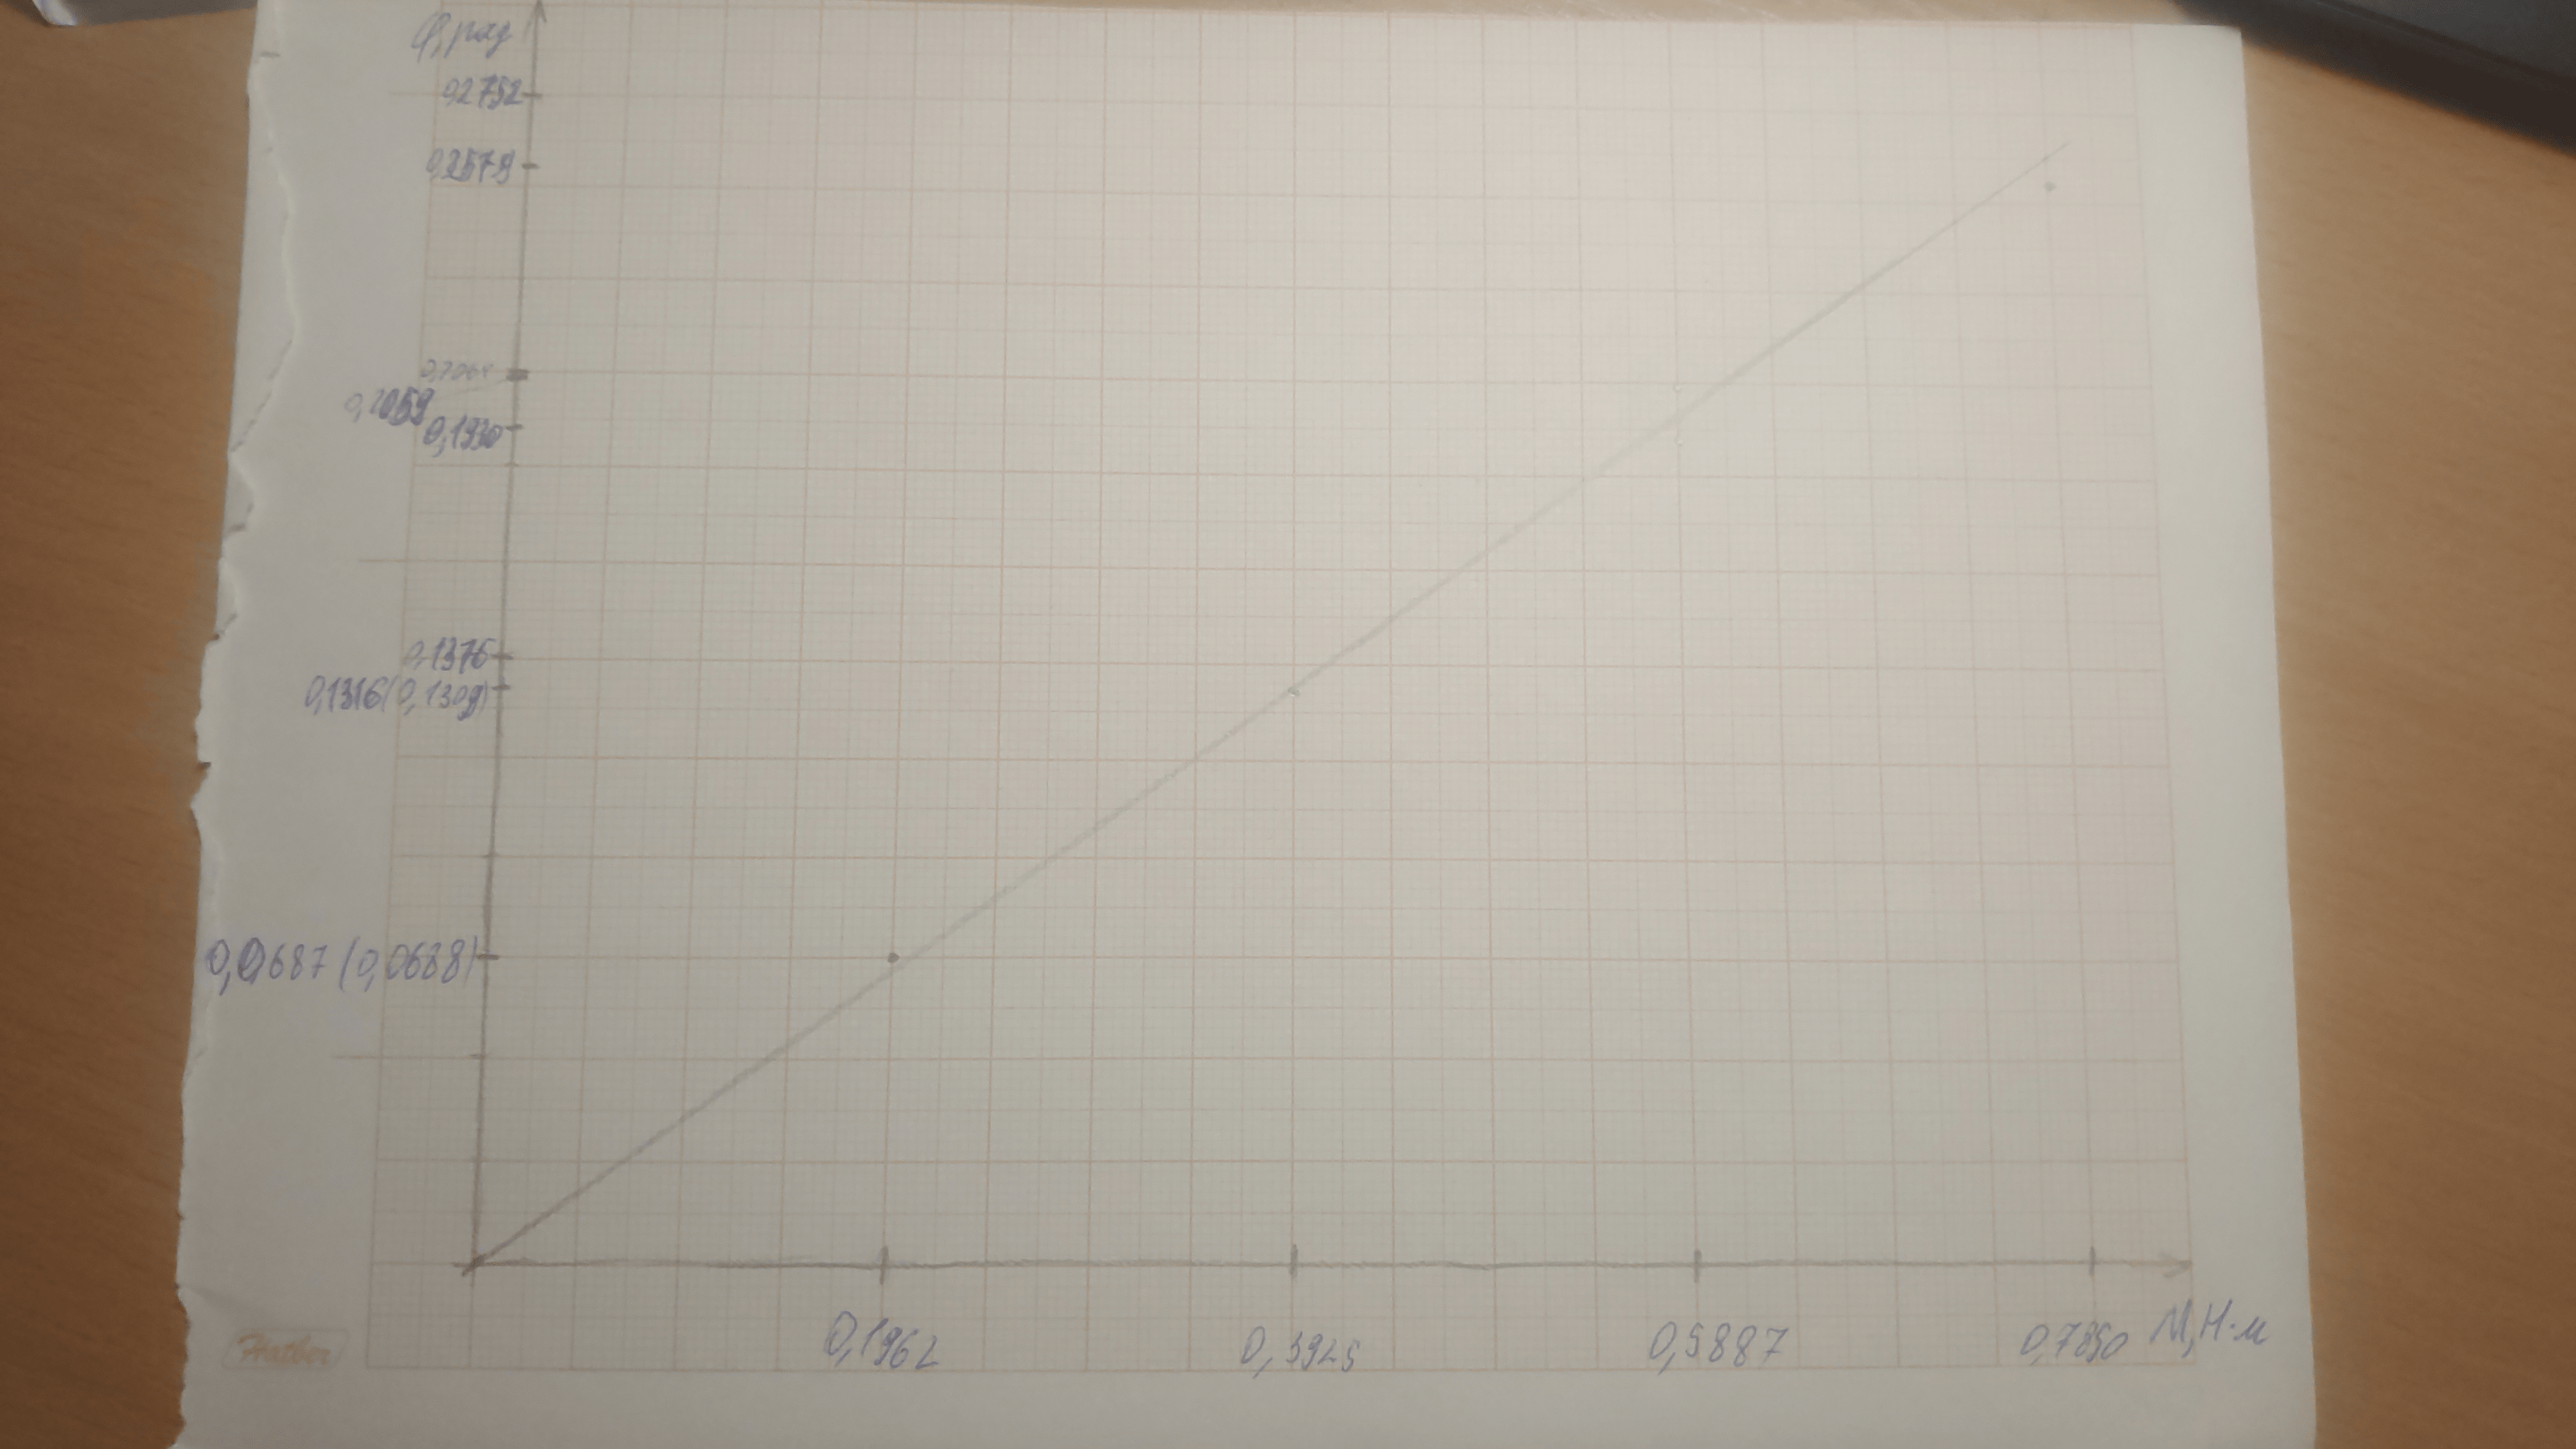
\includegraphics[scale=0.1]{Image2.png}
\caption{График зависимости $\varphi = \varphi(\textit{M})$}
\label{fig:Image1}
\end{figure}

\begin{center}
    \large
    \textbf{II. Определение модуля сдвига при помощи крутильных колебаний}
\end{center}    

Экспериментальная установка, используемая в этой части работы состоит из длинной горизонтально висящей проволоки, к нижнему концу которой прикреплен горизонтальный металлический стержень с двумя симметрично расположенными грузами. Их положение на стержне можно фиксировать. Верхний конец проволоки зажат в цангу и при помощи специального приспособления может вместе с цангой поворачиваться вокруг вертикальной оси. Таким способом в системе можно возбуждать крутильные колебания. Вращения стержня с закрепленными на нем грузами вокруг вертикальной оси происходит под действием упругого момента, возникающего в проволоке. Это вращение описывается уравнением:

\begin{equation}\label{8}
    I\frac{d^2 \varphi}{dt^2} = -M.
\end{equation}

Здесь $I$ - момент инерции стержня с грузами относительно оси вращения, $\varphi$ - угол поворота стержня от положения равновесия, $M$ - момент сил, действующий на стержень при закручивании проволоки, который при малых закручиваниях (малых $\varphi$) описывается формулой (\ref{6}). Вводим обозначение

\begin{equation}\label{9}
    \omega^2 = \frac{f}{I}
\end{equation}

При этом из (\ref{6}) и (\ref{8}) получаем

\begin{equation}\label{10}
    \frac{d^2 \varphi}{dt^2} + \omega^2\varphi =0
\end{equation}

Это уравнение гармонических колебаний. Его решение имеет вид

\begin{equation}\label{11}
    \varphi = \varphi_0\sin(\omega t + \theta).
\end{equation}

Здесь амплитуда $\varphi_0$ и фаза $\theta$ определяются начальными условиями. Период колебаний $T$ равен

\begin{equation}\label{12}
    T = \frac{2\pi}{\omega} = 2\pi\sqrt{\frac{I}{f}}.
\end{equation}

Уравнение (\ref{10}) и, следовательно (\ref{11}) и (\ref{12}) получены для незатухающих колебаний. Для их применения необходимо убедиться, что в рассматриваемом случае затуханием колебаний, то есть необратимыми потерями энергии, можно пренебречь. Если после 10 периодов колебаний, амплитуда уменьшается меньше, чем в 2 раза, то можно пользоваться результатами для незатухающих колебаний. Кроме того, следует убедиться, что период колебаний не зависит от начальной амплитуды. Начальную амплитуду нужно уменьшать до тех пор, пока не исчезнет зависимотсь периода от амплитуды.

\vspace{0,5cm}

\textbf{1.} Установим диапазон амплитуд, в котором применимы результаты, полученные для незатухающих колебаний. Также убедимся в том, что после десяти периодов колебаний амплитуда уменьшается менее, чем в два раза. Установим грузы на стержне на одинаковом расстоянии от проволоки, до центра масс каждого груза. Проведем измерения для различных \textit{l}, где \textit{l} - это расстояние от проволоки до начала груза. 

\vspace{0,5cm}

\begin{tabular}{|c|c|c|c|c|c|c|c|}
\hline
$l$, см & 4,25 & 5,25 & 6,25 & 7,25 & 8,25 & 9,25 & 11,25 \\
\hline
$T$, с & 2,168 & 2,505 & 2,668 & 2,906 & 3,171 & 3,407 & 3,981 \\
\hline
$T$, с & 2,127 & 2,491 & 2,670 & 2,926 & 3,153 & 3,415 & 3,962 \\
\hline
$T$, с & 2,146 & 2,473 & 2,593 & 2,951 & 3,091 & 3,456 & 4,001 \\
\hline
$T$, с & 2,173 & 2,469 & 2,629 & 2,883 & 3,184 & 3,388 & 3,958 \\
\hline
$T$, с & 2,118 & 2,502 & 2,679 & 2,946 & 3,157 & 3,421 & 3,974 \\
\hline
$T$, с & 2,100 & 2,482 & 2,632 & 2,913 & 3,133 & 3,472 & 3,997 \\
\hline
\end{tabular}

\vspace{0,5cm}

Погрешность измерения расстояния здесь будет определяться характеристиками линейки:

\[\sigma_l = 0,1\:\text{см}\]

Вычислим средние значения \textit{T} по формуле (\ref{13}) и случайную погрешность $\sigma_T$ по формуле (\ref{14}) для каждой длиы \textit{l} и занесем результаты в таблицу:

\vspace{0,5cm}

\begin{tabular}{|c|c|c|c|c|c|c|c|}
\hline
$l$, см & 4,25 & 5,25 & 6,25 & 7,25 & 8,25 & 9,25 & 11,25 \\
\hline
$T$, с & 2,139 & 2,487 & 2,645 & 2,921 & 3,148 & 3,427 & 3,979 \\
\hline
$\sigma_T$, с & 0,064 & 0,033 & 0,074 & 0,057 & 0,074 & 0,070 & 0,040 \\
\hline
\end{tabular}

\vspace{0,5cm}

По полученным точкам построим график в координатах $l^2,\: T^2$, при помощи метода наименьших квадратов:

\[l^2 = k T^2\]

\[k = \frac{\langle l^2 T^2 \rangle}{\langle(T^2)^2\rangle}  = 0,140\]

\textbf{2.} Измерим длину проволоки $\textit{l}_{\text{пр}}$, диаметр проволоки $d_{\text{пр}}$ и размеры грузов (\textit{L} - длина груза и \textit{D} - диаметр груза):

\[\textit{l}_{\text{пр}} = 144\: \text{см} \quad \textit{D}_{\text{пр}} = 1,91\: \text{мм}\]

\[L = 4\: \text{см} \quad D = 4\: \text{см}\]

Зная диаметр груза можем найти его радиус \textit{R}:

\[R = 2\: \text{см}\]

Аналогично находим радиус проволоки $\textit{R}_{\text{пр}}$:

\[\textit{R}_{\text{пр}} = 0,96\: \text{мм}\] 

Погрешности найденных значений определяются характеристиками приборов и равны:

\[\sigma_{\textit{l}_{\text{пр}}} = 0,1\: \text{см} \quad \sigma_{\textit{R}_{\text{пр}}} = 0,05\: \text{мм}\]
\[\sigma_L = 0,01\: \text{см} \quad \sigma_R = 0,01\: \text{см}\]

По формуле (\ref{15}) находим наудем модуль кручения \textit{f}:

\[f = \frac{4\pi^2 I}{T^2}\],

Где момент инерции \textit{I} можем найти по формуле:

\[I = \frac{m}{L}\Big(\frac{R^2 L}{2} + \frac{1}{3}\big((l + L)^3 - l^3\big)\Big)\]

Здесь \textit{m} - масса грузика. Масса грузика $m _{\text{гр}} = 375$ гр. Изучим колебания стержня без грузов:

\vspace{0,5cm}

\begin{tabular}{|c|c|c|c|c|c|c|c|c|}
\hline
$T_0$, с & 1,145 & 1,131 & 1,121 & 1,155 & 1,144 & 1,134 & 1,128 & 1,129 \\
\hline
\end{tabular}

\vspace{0,5cm} 

Найдем среднее значение $\textit{T}_0$ и погрешность измерения $\sigma_{T_0}$:

\[T_0 = 1,136 \: \text{с} \quad \sigma_{T_0} = 0,01 \: \text{с}\]

Так как наша формула для измерения момента инерции не включает в себя массу стержня и его момент инерции (из-за сложностей в их вычислении), то мы можем использовать такую формулу:

\[I_1 - I_0 = \frac{T^2 f}{4\pi^2} - \frac{T_0^2 f}{4\pi^2} = I\],

где $\textit{I}_1$ - это полный момент инерции складывающийся из момента инерции грузиков и стержня.

Тогда модуль кручения \textit{f} можем найти по формуле:

\[f = \frac{4\pi^2I}{T^2 - T_0^2}\]

Так как у нас имеется большое количество значений используем МНК:

\[\frac{4\pi^2}{f} = \frac{\langle (T^2 - T_0^2) I\rangle}{\langle I^2\rangle}\]

Посчитаем моменты инерции для различных длин и их погрешности по формуле:

\[\sigma_I = I\sqrt{3\Big(\frac{\sigma_L}{L}\Big) + 2\Big(\frac{\sigma_R}{R}\Big) + 3\Big(\frac{\sigma_l}{l}\Big) }\],

где $\sigma_l$ = 0,1 см.

Полученные данные занесем в таблицу:

\vspace{0,5cm}

\begin{tabular}{|c|c|c|c|c|c|c|c|c|}
\hline
$l$, см & 4,25 & 5,25 & 6,25 & 7,25 & 8,25 & 9,25 & 11,25 \\
\hline
$T$, с & 2,139 & 2,487 & 2,645 & 2,921 & 3,148 & 3,427 & 3,979 \\
\hline
$I$, $\text{кг}\cdot\text{м}^2$ & 0,0016 & 0,0021 & 0,0027 & 0,0033 & 0,0041 & 0,0049 & 0,0067 \\
\hline
$\sigma_I$, $\text{кг}\cdot\text{м}^2\cdot 10^{-5}$ & 6,65 & 7,14 & 7,81 & 8,35 & 9,25 & 10,03 & 11,72 \\
\hline
\end{tabular}

\vspace{0,5cm} 

При помощи данной таблицы определим модуль кручения \textit{f} и его погрешность:

\[f = 0,0316\:\text{Н}/\text{м}\]

\[\sigma_f = 8,2\cdot10^{-4} \:\text{Н}/\text{м}\]

Зная \textit{f} по формуле (\ref{7}) определим модуль сдвига \textit{G} и его погрешность:

\[G = \frac{2fl_{\text{пр}}}{\pi R_{\text{пр}}^4} = 3,407\cdot 10^{10} \:\text{Н}/\text{м}^2\]

\[\sigma_G = G\sqrt{4\Big(\frac{\sigma_{R_{\text{пр}}}}{R_{\text{пр}}}\Big)^2 + \Big(\frac{\sigma_{f}}{f}\Big)^2 + \Big(\frac{\sigma_{l_{\text{пр}}}}{l_{\text{пр}}}\Big)^2} = 2,2\cdot 10^9 \:\text{Н}/\text{м}^2\]

\textbf{Вывод:} расчитали модуль сдвига статическим и динамическим методом. Сравнив с табличными значениями определяем, что стержень и проволока сделаны из цинка, латуни или бронзы.

\end{document}